
\graphicspath{ {./Pictures/} }
%----------------------------------------------------------------------------------------
%	CHAPTER 3
%----------------------------------------------------------------------------------------

\chapterimage{boat.png}
\chapter{Calculus}
\section{Differentiation}

	In mathematics, differential calculus is a subfield of calculus concerned with the study of the rates at which quantities change.
	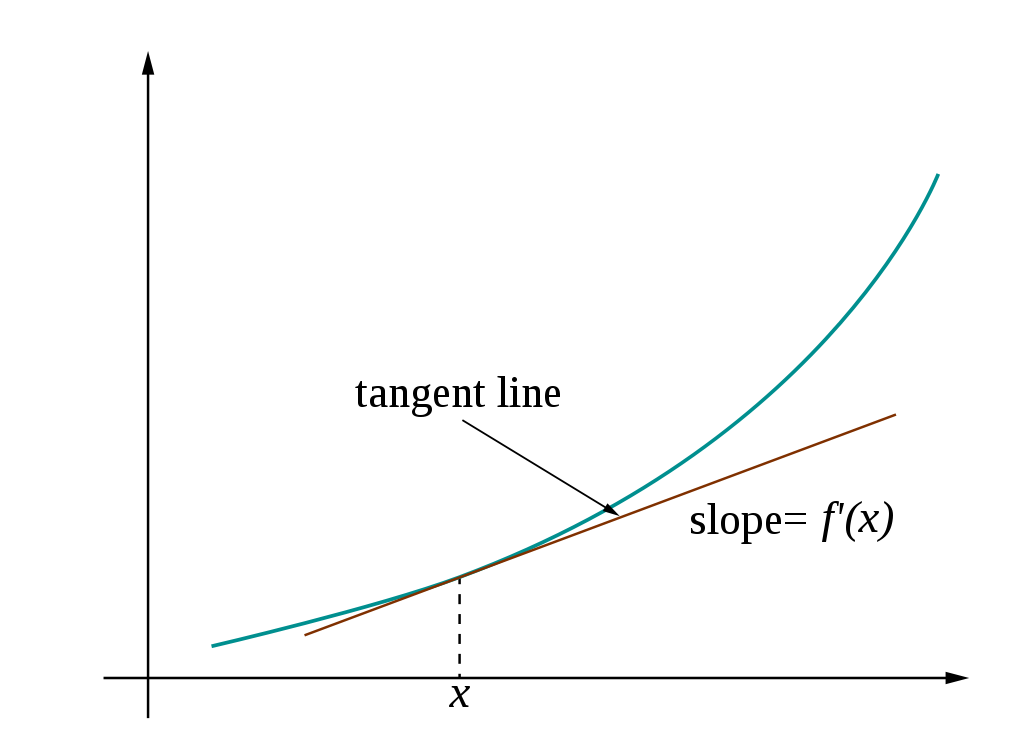
\includegraphics[width=50mm]{02}
	It is one of the two traditional divisions of calculus, the other being integral calculus, the study of the area beneath a curve.
	
	\begin{equation}
	\frac{duv}{dx}=\frac{du}{dx}v+u\frac{du}{dx}
	\end{equation}
	\begin{displaymath}
	\frac{df(x)}{dx} = \frac{f(x+h)-f(x)}{h}
	\end{displaymath}
	\begin{displaymath}
	=> \frac{(f+df)-(f)}{dx}
	\end{displaymath}
	\begin{displaymath}
	=>\frac{df}{dx}
	\end{displaymath}
	\newline
	\begin{displaymath}
	\frac{duv}{dx} = \frac{(u+du)(v+du)-uv}{dx}
	\end{displaymath}
	\begin{displaymath}
	=>\frac{(uv+du+udv+dudv)-uv}{dx}
	\end{displaymath}
	\begin{displaymath}
	=> \frac{duv+duv+dudv}{dx}
	\end{displaymath}
	\begin{displaymath}
	=> \frac{duv+udv}{dx}
	\end{displaymath}
	\begin{displaymath}
	=> \frac{du}{dx}v+u\frac{dv}{dx}
	\end{displaymath}
	\newline
	\begin{displaymath}
	\frac{df}{dx} = \frac{f_2-f_1}{x_2-x_1}
	\end{displaymath}
	\begin{displaymath}
	=>\frac{(f_1+df)-f_1}{x_2-x_1}
	\end{displaymath}
	\begin{displaymath}
	=>\frac{(f_1+df)-f_1}{dx}
	\end{displaymath}
	
	
	
	\subsection{Differentiation of trigonometric functions}
	\begin{equation}
	\sin(A+B) = \sin A\cos B+\cos A\sin B
	\end{equation}
	\begin{equation}
	\cos(A+B) = \cos A\cos B - \sin A\sin B
	\end{equation}
	\begin{equation}
	\frac{df(x)}{dx} = \frac{f(x+h)-x}{h}
	\end{equation}
	\newline
	Example: 1
	\begin{displaymath}
	\frac{d\sin(x)}{dx} = \frac{\sin x \cos h+\cos x\sin h-\sin x}{h}
	\end{displaymath}
	\begin{displaymath}
	=> \frac{\sin x + h\cos x - \sin x}{h}
	\end{displaymath}
	\begin{displaymath}
	=>\frac{h\cos x}{h}
	\end{displaymath}
	\begin{equation}
	\frac{d\sin(x)}{dx} = \cos x
	\end{equation}
	\newline
	Example: 2
	\begin{displaymath}
	\frac{d\cos(x)}{dx} = \frac{\cos(c+h)-\cos (x)}{h}
	\end{displaymath}
	\begin{displaymath}
	=> \frac{\cos x \cos h-\sin x \sin h - \cos x}{h}
	\end{displaymath}
	\begin{displaymath}
	=> \frac{cos x- h \cos x - \cos x}{h}
	\end{displaymath}
	\begin{displaymath}
	=> \frac{-h\sin x}{h}
	\end{displaymath}
	\begin{equation}
	\frac{d\cos (X)}{dx} = -\sin x
	\end{equation}
	\newline
	Example: 3
	\begin{displaymath}
	\frac{d\tan x}{dx}
	\end{displaymath}
	\begin{displaymath}
	=>\frac{d}{dx}\bigg(\frac{\sin x}{cos x}\bigg)
	\end{displaymath}
	\begin{displaymath}
	=>\frac{d}{dx}(\sin x)\frac{1}{\cos x}+\sin x \frac{d}{dx}\bigg(\frac{1}{\cos x}\bigg)
	\end{displaymath}
	\begin{displaymath}
	=>\cos x \frac{1}{\cos x}+\sin x\frac{d}{dx}(\cos x)^{-1}
	\end{displaymath}
	\begin{displaymath}
	=> 1+\sin x\bigg[(-1)(\cos x)^{-2}\frac{d\cos x}{dx}\bigg]
	\end{displaymath}
	\begin{displaymath}
	=> 1+\sin x\frac{-1}{\cos x^2}(-\sin x)
	\end{displaymath}
	\begin{equation}
	\frac{d \tan x}{dx} = 1 + \tan^2 x
	\end{equation}

	\subsection{Properties of Differential Operator}
	\subsection{Chain Rule}
	
	\begin{displaymath}
	\frac{df(g(x))}{dx} = \frac{df(g(x))}{dg(x)}\frac{dy(x)}{dx}
	\end{displaymath}
	\begin{equation}
	\frac{df(g(x))}{dx} = \frac{df(x)}{dy}\frac{dg(x)}{dx}
	\end{equation}
	\newline
	Example: 1
	\begin{equation}
	Proof\,that\, \quad\frac{de^{x^2}}{dx} = 2x \, e^{x^2}
	\end{equation}
	\begin{displaymath}
	Let, \quad x^2 = y
	\end{displaymath}
	\begin{displaymath}
	=> \frac{de^2}{dx}
	\end{displaymath}
	\begin{displaymath}
	=> \frac{de^y}{dy}\frac{dy}{dx}
	\end{displaymath}
	\begin{displaymath}
	e^y\frac{dx^2}{dx}
	\end{displaymath}
	\begin{displaymath}
	e^y\,2x
	\end{displaymath}
	\begin{displaymath}
	=> 2x\,e^{x^2}
	\end{displaymath}	
	\newline
	Example: 2
	\begin{displaymath}
	\frac{d\sin(x^3)}{dx}
	\end{displaymath}	 
	\begin{displaymath}
	=> \frac{d \sin(x^3)}{dx}\frac{d(x^3)}{dx}
	\end{displaymath}
	\begin{displaymath}
	=> \cos(x^3) \,3x^2
	\end{displaymath}
	\newline
	\begin{equation}
	\frac{d(2x^2)}{dx} = \frac{2(x+h)^2-2x^2}{h} = 2\Big[\frac{(x+h)^2-x^2}{h}\Big] = 2\frac{dx^2}{dx}=2.2x=4x
	\end{equation}
	\begin{equation}
	\frac{d(cf(x))}{dx} = c\frac{df(x)}{dx}\quad (c)\,\,is\,\,a\,\,number 
	\end{equation}
	\begin{equation}
	\frac{d}{dx}\bigg(c_1f(x)+c_2f(x)\bigg)=\frac{d}{dx}\bigg((c_1+c_2)f(x)\bigg)
	\end{equation}
	\begin{equation}
	\frac{d}{dx}\bigg(c_1u(x)+c_2v(x)\bigg)=c_1\frac{du(x)}{dx}+c_2\frac{dv(x)}{dx}
	\end{equation}
	c, are number. f(x), u(x), v(x) are function
	\newline
	\begin{equation}
	\frac{d\sin(2x^3)}{dx} = \frac{d\sin(2x^3)}{d2x^3}\frac{dx^3}{dx} = \cos(2x^3)\frac{2(x+h)^3-22x^3}{h}=\cos(2x^3)2\frac{dx^3}{dx}=\cos(2x^3)2\,3x^3=\cos(2x^3)6x^3
	\end{equation}
	\begin{equation}
	\frac{de^{\sin(3x)}}{dx}=\frac{de^{\sin(3x)}}{d\sin(3x)}\frac{d\sin(3x)}{dx}=e^{\sin(3x)}\frac{d\sin(3x)}{d3x}\frac{d3x}{dx} = e^{\sin(3x)}\cos(3x)3x
	\end{equation}
	
	\subsection{Differentiation of Fundamental Functions}
	(1) Differentiation Property:
	\begin{equation}
	\frac{d(uv)}{dx} = \frac{du}{dx}v+u\frac{du}{dx}
	\end{equation}
	\begin{equation}
	\frac{d}{dx}(uv)=\frac{du}{dx}v+u\frac{du}{dx}
	\end{equation}
	\begin{equation}
	\frac{d}{dx}(f(x)g(x)=\frac{df(x)}{dx}\bigg(g(x)+f(x)\frac{dg(x)}{dx}\bigg)
	\end{equation}
	\newline
	(2) Scalar multiplication:
	\begin{equation}
	\frac{dcf(x)}{dx} = c\frac{df(x)}{dx}
	\end{equation}
	d, c is a number or constant
	\begin{equation}
	\frac{d}{dx}\Big((x+d)u(x)\Big)=c\frac{du}{dx}+d\frac{du}{dx}
	\end{equation}
	\begin{equation}
	\frac{d}{dx}\Big(c(u+v)\Big) = c\frac{du}{dx} + c\frac{dv}{dx}
	\end{equation}

\section{Integration}
\subsection{Fundamental Theorem of Calculus}

\begin{equation}
\int_{a}^{b}f(x)dx=F(b)-F(a)
\end{equation}
\begin{equation}
\frac{dF(x)}{dx}=f(x)
\end{equation}

Derivative of F(x) gives the slope of F(x) at a point integration of (x) the area under carve in the range of integration.Here it is [a, b]
\newline
\begin{equation}
f(x_1)h+f(x_2)h+f(x_3)h
\end{equation}
\begin{equation}
\int f(x)dx=f(x_1)dx+f(x_2)dx+......+f(x_n)dx
\end{equation}
Example: 1
\begin{equation}
\frac{dx^n}{dx} = nx^{n-1}
\end{equation}
\begin{equation}
\frac{dx^2}{dx} = 2x => F(x)=x^2
\end{equation}
\begin{displaymath}
f(x) = 2x
\end{displaymath}
\begin{displaymath}
\int_{0}^{2}f(x)dx=\int_{0}^{2}(2x)dx = F(5)-F(0)
\end{displaymath}
\begin{displaymath}
=> x^2\prod_{0}^{2}
\end{displaymath}
\begin{displaymath}
=>2^2-0^2
\end{displaymath}
\begin{displaymath}
=>4
\end{displaymath}
\newline
\begin{equation}
Area \,\, of \,\, triangle\,\, = \frac{1}{2}(base)(height)
\end{equation}
\begin{displaymath}
=>\frac{1}{2}*2*4
\end{displaymath}
\begin{displaymath}
=> 4
\end{displaymath}
Note: Area of triangle bh = 1/2 bh+ 1/2 bh
\newline
Example: 2
\begin{equation}
\int_{0}^{\frac{\pi}{2}}\cos xdx = \sin\big(\frac{\pi}{2}\big) - \sin(0)
\end{equation}
Example: 3
\begin{equation}
\int e^x dx = e^x+c
\end{equation}
Example: 4
\begin{equation}
\int f(x)dx=F(x)+c
\end{equation}
\begin{equation}
\int x^3 dx = \frac{1}{4}x^3+c	
\end{equation}
\begin{displaymath}
\frac{1}{4}\frac{dx^4}{dx} = x^3
\end{displaymath}

\section{Taylor Series}

One of the most importent thing in physics
\begin{equation}
f(x) = f(x_0)+(x-x_0)\frac{f^\prime(x_0)}{1!}+(x-x_0)^2\frac{f^{\prime\prime}(x_0)}{2!}+(x-x_0)^3\frac{f^{\prime\prime\prime}(x_0)}{3!}+.......
\end{equation}
\begin{equation}
f(x) = a_0+a_1x+a_2x^2+a_3x^3+a_4x^4+........
\end{equation}
In taylor series we expand/express a function as a polynomial.
\newline
\begin{equation}
= f(x_0)+\frac{x-x_0}{1!}\frac{df(x)}{dx}+\frac{(x-x_0)^2}{2!}\frac{d^2f(x)}{dx^2}+\frac{(x-x_0)^3}{3!}\frac{d^3f(x)}{dx^3}+....
\end{equation}
\begin{equation}
(1).... \quad \frac{df(x)}{dx} = f^\prime(x)
\end{equation}
\begin{equation}
(2).... \quad \frac{d}{dx}\bigg(\frac{df(x)}{dx}\bigg) = \frac{d^2f(x)}{dx^2} = f^{\prime\prime}(x)
\end{equation}
\begin{equation}
(3).... \quad \frac{d}{dx}\bigg(\frac{d}{dx}\bigg(\frac{df(x)}{dx}\bigg)\bigg) = \frac{d^3f(x)}{dx^3} = f^{\prime\prime\prime}(x)
\end{equation}
\newpage
Example: 1
\begin{displaymath}
f(x) = e^x
\end{displaymath}
Expanding around, $ x_0 = 0 $	
\begin{displaymath}
f(x_0) = f(0) = e^0=1
\end{displaymath}
\begin{displaymath}
f^\prime(x_0)=f^\prime(0)=e^0=1
\end{displaymath}
\begin{displaymath}
f^{\prime\prime}(x_0)=f^{\prime\prime}(0)=e^0=1
\end{displaymath}
\begin{displaymath}
f^{\prime\prime\prime}(x_0)=f^{\prime\prime\prime}(0)=e^0=1
\end{displaymath}
\begin{displaymath}
so \,\, f(x) = e^x=1+\frac{(x-x_0)}{1!}+\frac{(x-0)^2}{2!}+\frac{(x-0)^3}{3!}+......
\end{displaymath}
\begin{displaymath}
e^x = 1 + x+\frac{x^2}{2!}+\frac{x^3}{3!}+\frac{x^4}{4!}+.......
\end{displaymath}
\newline
Example: 2
\begin{displaymath}
f(x) = \sin x
\end{displaymath}
Expanding Around $ x_0 = 0 $
\begin{displaymath}
f(0) = \sin 0 = 0
\end{displaymath}
\begin{displaymath}
f^\prime(x)=\cos x =f^\prime(0)=\cos 0 = 1
\end{displaymath}
\begin{displaymath}
f^{\prime\prime}(x)=-\sin x = f^{\prime\prime}(0)= -\sin x = 0
\end{displaymath}
\begin{displaymath}
f^{\prime\prime\prime}(x)=-\cos x = f^{\prime\prime\prime}(0)=-\cos 0 = -1
\end{displaymath}
\begin{displaymath}
f(x)=f(0)+xf^\prime(x_0)+\frac{x^2}{2!}f^{\prime\prime}(x_0)+\frac{x_3}{3!}f^{\prime\prime\prime}(x_0)+....
\end{displaymath}
\begin{displaymath}
\sin x = 0+x+0+\frac{x^3}{3!}(-1)+.....
\end{displaymath}
\begin{displaymath}
\sin x = x-\frac{x^3}{3!}+\frac{x^5}{5!}-\frac{x^7}{7!}+......
\end{displaymath}
\newline
Example: 3
\begin{displaymath}
f(x)= \cos x
\end{displaymath}
Expanding around $ x_0=0 $
\begin{displaymath}
f(x) = \cos 0 = 1
\end{displaymath}
\begin{displaymath}
f^\prime(x) = -\sin x = f^\prime(0)=-\sin(0) = 0
\end{displaymath}
\begin{displaymath}
f^{\prime\prime}(x) = - \cos x = f^{\prime\prime}(0)= -\cos(0) = -1
\end{displaymath}
\begin{displaymath}
f^{\prime\prime\prime}(x)= \sin x = f^{\prime\prime\prime}(0)=\sin(0)= 0
\end{displaymath}
\begin{displaymath}
f^{\prime\prime\prime\prime}(x)= \cos x = f^{\prime\prime\prime\prime}(0)=\cos x = 1
\end{displaymath}
\begin{displaymath}
f(x) = f(0)+xf^\prime(x_0)+\frac{x^2}{2!}f^{\prime\prime}(x_0)+\frac{x^3}{3!}f^{\prime\prime\prime}(x_0)+\frac{x^4}{4!}
f^{\prime\prime\prime\prime}(x_0)+.......
\end{displaymath}
\begin{displaymath}
\cos x = 1+0-\frac{x^2}{2!}(-1)+\frac{x^3}{3!}(0)-\frac{x^4}{4!}(+1)
\end{displaymath}
\begin{displaymath}
\cos x = 1-\frac{x^2}{2!}+\frac{x^4}{4!}-.........
\end{displaymath}

\section{Formula}
	\subsection{Differentiation}
	
	\begin{equation}
	\frac{dx^h}{dx} = hx^{h-1}
	\end{equation}
	\begin{equation}
	\frac{de^x}{dx} = e^x
	\end{equation}
	\begin{equation}
	\frac{da^x}{dx} = a^x \ln a
	\end{equation}
	\begin{equation}
	\frac{d\ln x}{dx} = \frac{1}{x}
	\end{equation}
	\begin{equation}
	\frac{d\log_a^x}{dx} = \frac{1}{x\ln a}
	\end{equation}
	\begin{equation}
	\frac{d\sin x}{dx} = \cos x
	\end{equation}
	\begin{equation}
	\frac{d\cos x}{dx} = -\sin x
	\end{equation}
	\begin{equation}
	\frac{dx^2}{dx} = 2x
	\end{equation}
	\begin{equation}
	\frac{dx^3}{dx} 3x^2
	\end{equation}
	
	\subsection{Integration}
	
	\begin{equation}
	n\int n^{n-1}dx=x^n+c
	\end{equation}
	\begin{equation}
	\int e^x dx = e^x+c
	\end{equation}
	\begin{equation}
	\ln \int a^x dx = a^x+c
	\end{equation}
	\begin{equation}
	\int \frac{1}{x}dx = \ln x+ c
	\end{equation}
	\begin{equation}
	\frac{1}{\ln(b)}\int \frac{1}{x}dx = \log_b^x+c
	\end{equation}
	\begin{equation}
	\int \cos dx = \sin x + c
	\end{equation}
	\begin{equation}
	-\int \sin x dx = \cos x + c
	\end{equation}
	Basically
	\newline
	\begin{equation}
	\int x ^n dx = \frac{x^{n-1}}{n+1}
	\end{equation}
	\begin{equation}
	\int e^x dx = e^x
	\end{equation}
	\begin{equation}
	\int a^x dx = \frac{a^x}{\ln a}
	\end{equation}
	\begin{equation}
	\int \frac{1}{x}dx = \ln a
	\end{equation}
	\begin{equation}
	\int \frac{1}{dx} = \log_b^{(x)}\ln (b)
	\end{equation}
	\begin{equation}
	\int \cos x dx = \sin x
	\end{equation}
	\begin{equation}
	\int \sin x dx = - \cos x
	\end{equation}

